%-----------------------------------------------------------------------
%\subsection{Mode and Level}
%-----------------------------------------------------------------------
%\tbc
%Baseliyos Jacob
\textbf{This paragraphs gives an overview about the input doducments used for the:}
\begin{itemize}
\item Analysis of the OBU Functions
\item Functional decomposition and allocation of macro- and microfunctions
\item Design of the OBU Functions
\item Determination of "Use Cases" and Szenarios for the different iteration of the Architecture and Design Document
\end{itemize} 

\textbf{The listed kind of documents will be used for the design:}

\begin{itemize}
\item\textbf{ERA TSI CCS Documents}
\item\textbf{openETCS API Spec}
\item\textbf{openETCS Requirements WP 2}
\item\textbf{Railway Operator Documents}
\item\textbf{Industry Documents}
\item\textbf{ERSA Simulator Documents}
\item\textbf{Other Project Partner Data information and documents}
\item\textbf{Utrecht - Amsterdam Track Documents}
\end{itemize}

\textbf{Furthermore relevant ETCS Know How from Industry and Operator is used for the design and the analysis}

\textbf{The list and links to the relevant documents will be maintained and can be downloaded on to following link:}
\url{https://github.com/openETCS/modeling/wiki/Input-Documents-Repository}
and the link to the documents used in the standard \url{https://github.com/openETCS/SSRS/wiki/SSRS-Documents}

The figure below will demonstrate the use, filtering and proceeding of the input documents for the analyisis\\

\begin{figure}[h]
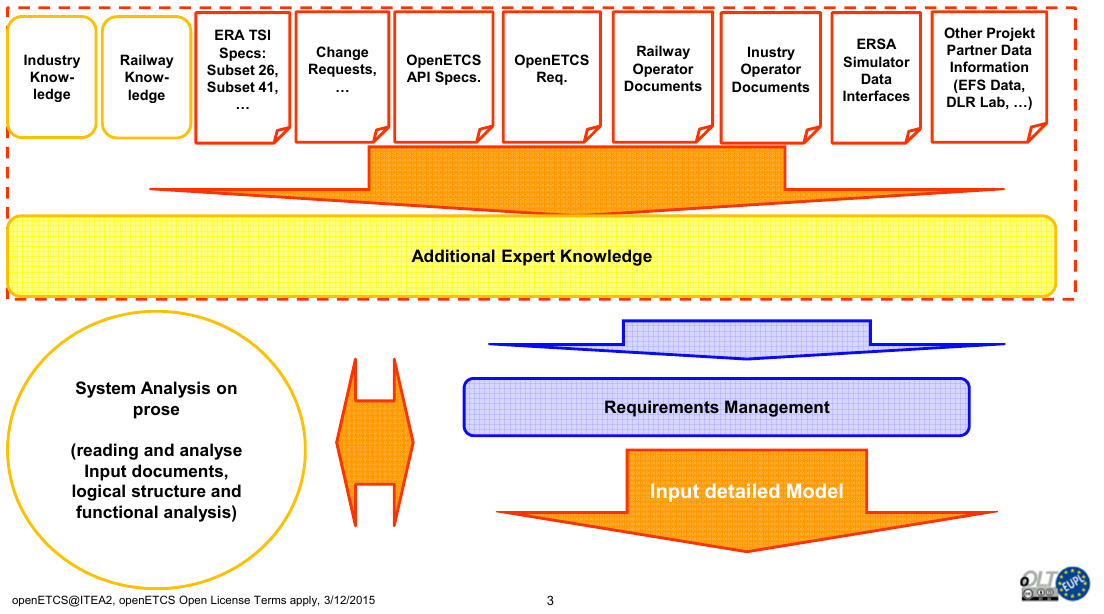
\includegraphics[scale=0.5]{images/AnalysisDocuments}
\caption{Analysing of input document}
\label{Analyising of input document}
\end{figure}